\documentclass[12pt,twoside]{article}

\textwidth 17cm \textheight 25cm \evensidemargin 0cm
\oddsidemargin 0cm \topmargin -2cm
\parindent 0pt
%\parskip \bigskipamount

\usepackage{graphicx}
\usepackage[dutch]{babel}
\usepackage{amssymb,amsthm,amsmath}
%\usepackage{dot2texi}
\usepackage[utf8]{inputenc}
\usepackage{nopageno}
\usepackage{pdfpages}
\usepackage{enumerate}
\usepackage{caption}
\usepackage{wrapfig}
\usepackage{pgf,tikz,pgfplots}
\pgfplotsset{compat=1.15}
\usepackage{color}
\usetikzlibrary{arrows}
\usetikzlibrary{patterns}
\usepackage{fancyhdr}
\pagestyle{fancy}
\usepackage[version=3]{mhchem}
\usepackage{multicol}
\usepackage{fix-cm}
\usepackage{setspace}
\usepackage{mhchem}
\usepackage{xhfill}
\usepackage{parskip}
\usepackage{cancel}
\usepackage{mdframed}
\usepackage{url}
\usepackage{mathtools}
\usepackage{changepage}

\newcommand{\todo}[1]{{\color{red} TODO: #1}}

\newcommand{\degree}{\ensuremath{^\circ}}
\newcommand\rad{\qopname\relax o{\mathrm{rad}}}

\newcommand\ggd{\qopname\relax o{\mathrm{ggd}}}

\pgfmathdeclarefunction{gauss}{2}{%
  \pgfmathparse{1/(#2*sqrt(2*pi))*exp(-((x-#1)^2)/(2*#2^2))}%
}

\def\LRA{\Leftrightarrow}

\newcommand{\zrmbox}{\framebox{\phantom{EXE}}\phantom{X}}
\newcommand{\zrm}[1]{\framebox{#1}}

% environment oefening:
% houdt een teller bij die de oefeningen nummert, probeert ook de oefening op één pagina te houden
\newcounter{noefening}
\setcounter{noefening}{0}
\newenvironment{oefening}
{
  \stepcounter{noefening}
  \pagebreak[0]
  \begin{minipage}{\textwidth}
  \vspace*{0.7cm}{\large\bf Oefening \arabic{noefening}}
}{%
  \end{minipage}
}

\usepackage{calc}

% vraag
\reversemarginpar
\newcounter{punten}
\setcounter{punten}{0}
\newcounter{nvraag}
\setcounter{nvraag}{1}
\newlength{\puntwidth}
\newlength{\boxwidth}
\newcommand{\vraag}[1]{
\settowidth{\puntwidth}{\Large{#1}}
\setlength{\boxwidth}{1.5cm}
\addtolength{\boxwidth}{-\puntwidth}
{\large\bf Vraag \arabic{nvraag} \addtocounter{nvraag}{1}}\vspace*{-0.5cm}
{\marginpar{\color{lightgray}\fbox{\parbox{1.5cm}{\vspace*{1cm}\hspace*{\boxwidth}{\Large{#1}}}}}
\vspace*{0.5cm}}
\addtocounter{punten}{#1}}

% arulefill
\def\arulefill{\leavevmode{\xrfill[-5pt]{0.3pt}[lightgray]\endgraf}\vspace*{0.2cm}}

% \arules{n}
\newcommand{\arules}[1]{
\color{lightgray}
%\vspace*{0.05cm}
\foreach \n in {1,...,#1}{
  \vspace*{0.75cm}
  \hrule height 0.3pt\hfill
}\color{black}\vspace*{0.2cm}}

% \arule{x}
\newcommand{\arule}[1]{
\color{lightgray}{\raisebox{-0.1cm}{\rule[-0.05cm]{#1}{0.3pt}}}\color{black}
}

% \abox{y}
\newcommand{\abox}[1]{
\fbox{
\begin{minipage}{\textwidth- 4\fboxsep}
\hspace*{\textwidth}\vspace{#1}
\end{minipage}
}
}

\newcommand{\ruitjes}[1]{
\definecolor{cqcqcq}{rgb}{0.85,0.85,0.85}
\hspace*{-2.5cm}
\begin{tikzpicture}[scale=1.04,line cap=round,line join=round,>=triangle 45,x=1.0cm,y=1.0cm]
\draw [color=cqcqcq, xstep=0.5cm, ystep=0.5cm] (0,-#1) grid (20.5,0);
\end{tikzpicture}
}


\newcommand{\assenstelsel}[5][1]{
\definecolor{cqcqcq}{rgb}{0.65,0.65,0.65}
\begin{tikzpicture}[line cap=round,line join=round,>=triangle 45,x=#1cm,y=#1cm]
\draw [color=cqcqcq,dash pattern=on 1pt off 1pt, xstep=1.0cm,ystep=1.0cm] (#2,#4) grid (#3,#5);
\draw[->,color=black] (#2,0) -- (#3,0);
%\draw[shift={(1,0)},color=black] (0pt,2pt) -- (0pt,-2pt) node[below] {\footnotesize $1$};
%\draw[color=black] (#3.25,0.07) node [anchor=south west] {$x$};
\draw[->,color=black] (0,#4) -- (0,#5);
%\draw[shift={(0,1)},color=black] (2pt,0pt) -- (-2pt,0pt) node[left] {\footnotesize $1$};
\draw[color=black] (0.09,#5.25) node [anchor=west] {\phantom{$y$}};
%\draw[color=black] (0pt,-10pt) node[right] {\footnotesize $0$};
\end{tikzpicture}
}

\newcommand{\getallenas}[3][1]{
\definecolor{cqcqcq}{rgb}{0.65,0.65,0.65}
\begin{tikzpicture}[scale=#1,line cap=round,line join=round,>=triangle 45,x=1.0cm,y=1.0cm]
\draw [color=cqcqcq,dash pattern=on 1pt off 1pt, xstep=1.0cm,ystep=1.0cm] (#2,-0.2) grid (#3,0.2);
\draw[->,color=black] (#2.25,0) -- (#3.5,0);
\draw[shift={(0,0)},color=black] (0pt,2pt) -- (0pt,-2pt) node[below] {\footnotesize $0$};
\draw[shift={(1,0)},color=black] (0pt,2pt) -- (0pt,-2pt) node[below] {\footnotesize $1$};
\draw[color=black] (#3.25,0.07) node [anchor=south west] {$\mathbb{R}$};
\end{tikzpicture}
}

\newcommand{\visgraad}[1]{\begin{tabular}{p{0.5cm}|p{#1}}&\\\hline\\\end{tabular}}

\newcommand{\tekenschema}[2]{\begin{tabular}{p{0.5cm}|p{#1}}&\\\hline\\[#2]\end{tabular}}

% schema van Horner
\newcommand{\schemahorner}{
\begin{tabular}{p{0.5cm}|p{7cm}}
&\\[1.5cm]
\hline\\
\end{tabular}}

% geef tabular iets meer ruimte
\setlength{\tabcolsep}{14pt}
\renewcommand{\arraystretch}{1.5}

\newcommand{\toets}[3]{
\thispagestyle{plain}
\vspace*{-2.5cm}
\begin{tikzpicture}[remember picture, overlay]
    \node [shift={(15.25 cm,-1.6cm)}] {%
        \includegraphics[width=1.8cm]{/home/ppareit/kaa1415/logokaavelgem.png}%
    };%
\end{tikzpicture}

\begin{tabular}{|llc|c|}
\hline
\vspace*{-0.5cm}
&&&\\
Naam & \arule{4cm} & {\Large\bf KA AVELGEM} & \\
\vspace*{-0.75cm}
&&&\\
Klas & \arule{4cm} & {\Large\bf 20...-...-...} & \\
\hline
\vspace*{-0.75cm}
&&&\\
Toets & {\bf #2} & {\large\bf #1} & Beoordeling\\
\vspace*{-0.75cm}
&&&\\
Onderwerp & \multicolumn{2}{l|}{\bf #3} &\\
\hline
\end{tabular}
}

\newcommand{\oefeningen}[1]{

\fancyhead[LE, RO]{\vspace{0.5cm} #1}
%\thispagestyle{plain}

{\bf \Large \centering Oefeningen: #1}

}

\raggedbottom

\newcommand\vl{\qopname\relax o{\mathrm{vl}}}

\newcommand\dom{\qopname\relax o{\mathrm{dom}}}
\newcommand\ber{\qopname\relax o{\mathrm{ber}}}

\newcommand\mC{\qopname\relax o{\mathrm{mC}}}
\newcommand\uC{\qopname\relax o{\mathrm{{\mu}C}}}
\newcommand\C{\qopname\relax o{\mathrm{C}}}

\newcommand\W{\qopname\relax o{\mathrm{W}}}
\newcommand\kW{\qopname\relax o{\mathrm{kW}}}
\newcommand\kWh{\qopname\relax o{\mathrm{kWh}}}


\newcommand\V{\qopname\relax o{\mathrm{V}}}
\newcommand\ohm{\qopname\relax o{\mathrm{\Omega}}}
\newcommand\kohm{\qopname\relax o{\mathrm{k\Omega}}}


\newcommand\N{\qopname\relax o{\mathrm{N}}}

\newcommand\Nperkg{\qopname\relax o{\mathrm{N/kg}}}

\newcommand\Nperm{\qopname\relax o{\mathrm{N/m}}}

\newcommand\gpermol{\qopname\relax o{\mathrm{g/mol}}}


\newcommand\kgperm{\qopname\relax o{\mathrm{kg/m}}}
\newcommand\kgperdm{\qopname\relax o{\mathrm{kg/dm}}}
\newcommand\gpercm{\qopname\relax o{\mathrm{g/cm}}}
\newcommand\gperml{\qopname\relax o{\mathrm{g/ml}}}


\newcommand{\mA}{\;\mbox{mA}}
\newcommand{\A}{\;\mbox{A}}
\newcommand{\MA}{\;\mbox{MA}}

\newcommand{\us}{\;\mu\mbox{s}}
\newcommand\s{\qopname\relax o{\mathrm{s}}}

\newcommand\h{\qopname\relax o{\mathrm{h}}}

\newcommand{\kmperh}{\;\mbox{km/h}}
\newcommand{\mpers}{\;\mbox{m/s}}
\newcommand{\kmpermin}{\;\mbox{km/min}}
\newcommand{\kmpers}{\;\mbox{km/s}}

\newcommand{\mph}{\;\mbox{mph}}

\newcommand{\Hz}{\;\mbox{Hz}}

\newcommand\Gm{\qopname\relax o{\mathrm{Gm}}}
\newcommand\Mm{\qopname\relax o{\mathrm{Mm}}}
\newcommand\km{\qopname\relax o{\mathrm{km}}}
\newcommand\hm{\qopname\relax o{\mathrm{hm}}}
\newcommand\dam{\qopname\relax o{\mathrm{dam}}}
\newcommand\m{\qopname\relax o{\mathrm{m}}}
\newcommand\dm{\qopname\relax o{\mathrm{dm}}}
\newcommand\cm{\qopname\relax o{\mathrm{cm}}}
\newcommand\mm{\qopname\relax o{\mathrm{mm}}}
\newcommand\um{\qopname\relax o{\mathrm{{\mu}m}}}
\newcommand\nm{\qopname\relax o{\mathrm{nm}}}


\newcommand\Gg{\qopname\relax o{\mathrm{Gg}}}
\newcommand\Mg{\qopname\relax o{\mathrm{Mg}}}
\newcommand\kg{\qopname\relax o{\mathrm{kg}}}
\newcommand\hg{\qopname\relax o{\mathrm{hg}}}
\renewcommand\dag{\qopname\relax o{\mathrm{dag}}}
\newcommand\g{\qopname\relax o{\mathrm{g}}}
\newcommand\dg{\qopname\relax o{\mathrm{dg}}}
\newcommand\cg{\qopname\relax o{\mathrm{cg}}}
\newcommand\mg{\qopname\relax o{\mathrm{mg}}}
\newcommand\ug{\qopname\relax o{\mathrm{{\mu}g}}}
\renewcommand\ng{\qopname\relax o{\mathrm{ng}}}

\newcommand\ton{\qopname\relax o{\mathrm{ton}}}

\newcommand\Gl{\qopname\relax o{\mathrm{Gl}}}
\newcommand\Ml{\qopname\relax o{\mathrm{Ml}}}
\newcommand\kl{\qopname\relax o{\mathrm{kl}}}
\newcommand\hl{\qopname\relax o{\mathrm{hl}}}
\newcommand\dal{\qopname\relax o{\mathrm{dal}}}
\renewcommand\l{\qopname\relax o{\mathrm{l}}}
\newcommand\dl{\qopname\relax o{\mathrm{dl}}}
\newcommand\cl{\qopname\relax o{\mathrm{cl}}}
\newcommand\ml{\qopname\relax o{\mathrm{ml}}}
\newcommand\ul{\qopname\relax o{\mathrm{{\mu}l}}}
\newcommand\nl{\qopname\relax o{\mathrm{nl}}}

\newcommand\MJ{\qopname\relax o{\mathrm{MJ}}}
\newcommand\kJ{\qopname\relax o{\mathrm{kJ}}}
\newcommand\J{\qopname\relax o{\mathrm{J}}}

\newcommand\T{\qopname\relax o{\mathrm{T}}}
\newcommand\uT{\qopname\relax o{\mathrm{{\mu}T}}}

\newcommand\grC{\qopname\relax o{\mathrm{{\degree}C}}}

\newcommand\K{\qopname\relax o{\mathrm{K}}}
\newcommand\calperK{\qopname\relax o{\mathrm{cal/K}}}

\newcommand\hPa{\qopname\relax o{\mathrm{hPa}}}
\newcommand\Pa{\qopname\relax o{\mathrm{Pa}}}

\newcommand\dB{\qopname\relax o{\mathrm{dB}}}

\newcommand\Var{\qopname\relax o{\mathrm{Var}}}

\newcommand{\EE}[1]{\cdot 10^{#1}}

\onehalfspacing

%\setlength{\headsep}{0cm}

\newenvironment{exlist}[1] %
{ \begin{multicols}{#1}
  \begin{enumerate}[(a)]
    \setlength{\itemsep}{0.5em} }
{ \end{enumerate}
  \end{multicols} }




\usepackage{pgfplots}

\usepackage{relsize}


\usepackage{versions}
\excludeversion{theorie}
%\includeversion{theorie}

\newtheorem{definition}{Definitie}
\newtheorem{eigenschap}{Eigenschap}

% vergelijkingen mooi uitlijnen:
% \begin{alignat}{2}
%   &&    a^2-b^2 &= 0\\
%   \lra && (a-b)(a+b) &= 0\\
% \end{alignat}
\newcommand{\lra}{\ensuremath{\Leftrightarrow\qquad}}



\begin{document}

\pagestyle{fancy}
\lhead{}
\rhead{Oefeningen Veeltermfuncties}

\begin{theorie}
\thispagestyle{empty}
\begin{center}
  \begin{mdframed}
  \centering
  \fontsize{40}{60}\selectfont Veeltermfuncties
  \end{mdframed}
  \vfill
  \vfill
\end{center}

\subsection*{Doelstellingen}
\vspace*{-0.8cm}
{\singlespacing
Je \hfill  {\scriptsize(LP2006-059, LI1.1, ET14)}
\begin{itemize}
\end{itemize}}

\thispagestyle{empty}
\mbox{}
\newpage
\clearpage
\thispagestyle{empty}
%\mbox{}
\tableofcontents
\newpage
\clearpage
\pagenumbering{arabic} 

\fancyhead[RO,LE]{Veeltermfuncties}
\fancyhead[RE,LO]{}

\end{theorie}

\onehalfspacing

\pagebreak

\section{Veeltermvergelijking}

\begin{oefening}
  Los de volgende vergelijkingen van de eerste graad op in $\mathbb{R}$
  \begin{multicols}{2}
    \begin{enumerate}[(a)]
      \itemsep0.7em
    \item $4x-8=0$
    \item $3x+9=0$
    \item $-3x+9=0$
    \item $2(x+6)=4-(x+7)$
    \item $x - \dfrac{x-2}{3} = 4$
    \item $2(x-3)+7=5-(2-x)$
    \item $(x+1)^2-2=x(x-3)-(1-2x)$
    \item $\dfrac{3+2x}{4}-\dfrac{4x-5}{5}=\dfrac{21-6x}{6}$
    \item $\dfrac{4x}{3}-\left(\dfrac{3}{2}-\dfrac{x}{4}\right)=x+4\left(\dfrac{2x}{3}-1\right)$
    \item $\dfrac{3(x-1)}{5}-\dfrac{2(1-4x)}{7}=x+\dfrac{x+1}{5}$
    \item $\dfrac{5x}{8}-\dfrac{x-\frac{5}{2}}{4}=1$
    \item $\dfrac{x}{5}+\dfrac{x}{2}=-7$
    \item $\dfrac{3-x}{4}-\dfrac{x-2}{3}=\dfrac{x}{2}-\dfrac{4x+1}{12}$
    \end{enumerate}
  \end{multicols}
\end{oefening}

\begin{oefening}
  Los de volgende vergelijkingen van de tweede graad op in $\mathbb{R}$
  \begin{multicols}{2}
    \begin{enumerate}[(a)]
      \itemsep0.7em
    \item $2x^2-4x-6=0$
    \item $5x(x-2)=x(3x-4)-5$
    \item $\frac{2}{3}x^2+5x+1=0$
    \item $80x^2+8x=15$
    \item $80x^2+15=-8x$
    \item $(3-x)(3+x)=(x-4)^2$
    \item $(x-2)^2=x^2-4$
    \item $(3x+2)(3x-2)+6x+5=0$
    \item $x+1=(x+1)(x-1)$
    \item $4x^2-20x+25=0$
    \item $3x^2+5=0$
    \item $x=x^2$
    \item $2\left(7x+32\right)=(3x+8)^2$
    \item $11x+13=2x^2$
    \item $x\left(x+3\right)+2\left(5+2x\right)=0$
    \item $x^2+2x-8=0$
    \item $(x+3)^2=16$
    \item $9x^2+30x+25=0$
    \item $10x^2+7x-3=0$
    \item $x^2=x+1$
    \item $37x^2+13x-50=0$
    \item $3x(3x+10)+5=-20$
    \item $x^2=3x-18$
    \item $x^2=10x-25$
    \end{enumerate}
  \end{multicols}
\end{oefening}

\begin{oefening}
  Los op in $\mathbb{R}$
  \begin{enumerate}[(a)]
      \itemsep1em
    \item $x^2+x-8=(x-6)^2$% \tabto{6cm} {\color{gray}$V=\{\dfrac{44}{13}\}$}
    \item $x^2+\dfrac{15}{2}=\dfrac{11x}{2}$% \tabto{6cm} {\color{gray}$V=\{\dfrac{5}{2}, 3\}$}
    \item $(2x-4)(2x+4)=(x+2)^2$% \tabto{6cm} {\color{gray}$V=\{-2,\dfrac{10}{3}\}$}
    \item $9x^2-36=(6+3x)^2$% \tabto{6cm} {\color{gray}$V=\{-2\}$}
    \item $19-x+x^2=18-2x-x^2$% \tabto{6cm} {\color{gray}$V=\{\}$}
    \item $25x^2+20x=-9$% \tabto{6cm} {\color{gray}$V=\{-\dfrac{3}{5}\}$}
    \item $6x^2=x+1$% \tabto{6cm} {\color{gray}$V=\{-\dfrac{1}{3},\dfrac{1}{2}\}$}
  \end{enumerate}
\end{oefening}

\begin{oefening}
De ring links en de cirkel rechts hebben dezelfde oppervlakte. Bepaal $x$.
\begin{center}
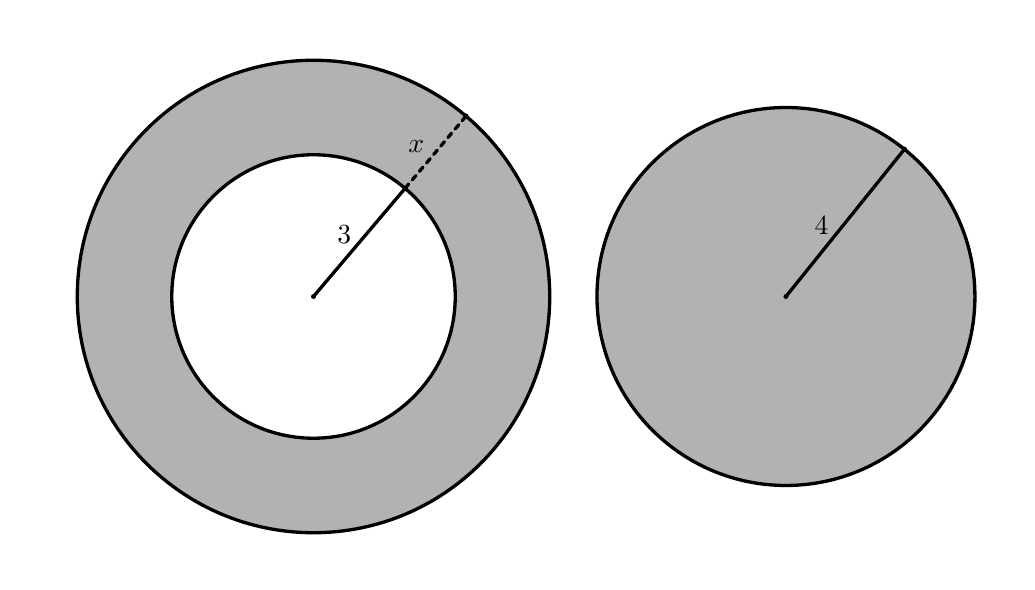
\begin{tikzpicture}[scale=0.6, line cap=round,line join=round,>=triangle 45,x=1.0cm,y=1.0cm]
\clip(-2.05,-0.62) rectangle (18.68,10.69);
\draw [line width=1.2pt,fill=gray!60] (4,5) circle (5cm);
\draw [line width=1.2pt,fill=white] (4,5) circle (3cm);
\draw [line width=1.2pt,fill=gray!60] (14,5) circle (4cm);
\draw [line width=1.2pt] (14,5)-- (16.51,8.12);
\draw [line width=1.2pt] (4,5)-- (5.94,7.29);
\draw [line width=1.2pt,dash pattern=on 2pt off 2pt] (5.94,7.29)-- (7.23,8.82);
\draw (5.8,8.5) node[anchor=north west] {$x$};
\draw (4.3,6.7) node[anchor=north west] {3};
\draw (14.4,6.9) node[anchor=north west] {4};
\fill [color=black] (4,5) circle (1.5pt);
\fill [color=black] (14,5) circle (1.5pt);
\fill [color=black] (7.23,8.82) circle (1.5pt);
\fill [color=black] (16.51,8.12) circle (1.5pt);
\fill [color=black] (5.94,7.29) circle (1.5pt);
\end{tikzpicture}
\end{center}
\end{oefening}

\begin{oefening}
  Los op in $\mathbb{R}$
  \begin{multicols}{2}
    \begin{enumerate}[(a)]
    \itemsep0.7em
    \item $x^3+2x-3=0$
    \item $7x^3+8x^2+3x+2=0$
    \item $x^3-x+6=0$
    \item $3x^2(x-1)=\dfrac{7}{2}x^2-2$
    \item $8x^3+12x^2+6x+2=0$
    \item $20x^3+60x^2+45x=0$
    \item $x^4-4x^3-x^2+16x-12=0$
    \item $x+\dfrac{7x}{2}=\dfrac{3x^3}{2}+\dfrac{3x^2}{2}+\dfrac{3}{2}$
    \item $x^3+(2x+1)^2=x+1$
    \end{enumerate}
  \end{multicols}
\end{oefening}

\begin{oefening} % www3.ul.ie/~mlc/support/.../chap3/3_3.pdf
  Los volgende vergelijkingen van graad hoger dan twee op in $\mathbb{R}$:
  \begin{multicols}{2}
  \begin{enumerate}[(a)]
  \itemsep.7em
  \item $x^3-17x^2+54x-8=0$
  \item $x^3-6x^2+11x-6=0$
  \item $x^3-7x=6$
  \item $2x^3+9x^2+7x+2=2x^2$
  \item $22x+8=3x^3+7x^2$
  \item $2x^4+8x^3-\dfrac{7x^2}{2}-\dfrac{67x}{2}-15=0$
  \item $4x^4+8x^3+3x^2-2x-1=0$
  \end{enumerate}
  \end{multicols}
\end{oefening}

\begin{oefening}
Los op in $\mathbb{R}$:
\begin{enumerate}[(a)]
  \itemsep0.6em
  \begin{multicols}{2}
  \item $2x^3+3x^2-17x+12=0$
  \item $3x^3+13x^2-18x-40=0$
  \item $x^3+4x^2-15x-18=0$
  \item $2x^3+9x^2+7x-6=0$
  \item $-3x^3+16x^2-17x+4=0$
  \item $2x^4+3x^3=17x^2-12x$
  \item $16x^3+4x=3x^4+17x^2$
  \item $2x^4-11x^3-12x^2+36x=0$
  \item $x^4+3x^3-51x^2+37x+90=0$
  \item $6x^3-11x^2-3x+2=0$
  \item $x^3-9x^2+26x=24$
  \item $x^3-3x+2=0$
  \item $x^4+x^3=10x^2-8x$
  \item $x^4+2x-1=2x^3$
  \item $1=x^4$
  \item $3x^2+x(x-1)^2=5x+4$
  \item $(x+1)(x^2+2x+1)=2x(x+2)-1$
  \item $x^3+70=39x$
  \item $x^4+3x^2+10x=6x^3$
  \item $-2(10x+x^3)=x^2(10+x^2)$
  \item $x^4+82x+176=93x^2-2x^3$
  \item $12x^3+22x^2-6x-4=0$
  \item $2x(3x^3-26)=20+x^2(31-7x)$
  \item $x^4-8x^3-3x^2+62x+56=0$
  \item $-x^3+3x^2-3x=0$
  \item $-x^4-x^3-7x^2-9x+18=0$
  \end{multicols}
\end{enumerate}
\end{oefening}

\pagebreak
\section{Veeltermfuncties}

\begin{oefening}
Bespreek volgende functies:
\begin{multicols}{2}
\begin{enumerate}[(a)]
  \itemsep.5em
  \item $\displaystyle f(x)=42$
  \item $\displaystyle f(x)=0$
  \item $\displaystyle f(x)=-2x+3$
  \item $\displaystyle f(x)=\dfrac{1}{2}x-2$
  \item $\displaystyle f(x)=-x^2+7x-10$
  \item $\displaystyle f(x)=\dfrac{1}{4}x^2-x-3$
  \item $f(x)=(x+2)^2-4$
  \item $f(x)=4x+(x-2)^2$
  \item $f(x)=(x-2)(x+2)$
  \item $f(x)=(x+3)^2+(x-3)^2$
  \item $f(x)=-(x-1)(x+1)$
  \item $f(x)=-2x^2+29x-102$
\end{enumerate}
\end{multicols}
\end{oefening}

\begin{oefening}
Bepaal het functievoorschrift van
\begin{enumerate}[(a)]
  \itemsep.5em
  \item de rechte door $(-2, 3)$ en $(1, 0)$.
  \item de rechte door $(-2, 0)$ en $(1, 3)$.
  \item de rechte door $(1, -1)$ en $(3, -1)$.
  \item de rechte door $(3, -1)$ en $(3, 6)$.
  \item de parabool door $(1,4)$ en met nulwaarden 2 en 5.
  \item de parabool met volgende functiewaardentabel
  \begin{center}
    \begin{tabular}{c|cccccc}
    $x$ & -2 & -1 & 0 & 1 & 2 & 3\\
    \hline
    $y$ & 2.25 & -1.75 & -3.75 & -3.75 & -1.75 & 2.25
    \end{tabular}
  \end{center}
\end{enumerate}
\end{oefening}

\begin{oefening}
Bespreek (domein, bereik, nulwaarden, tekenverloop, schets, stijgen\&dalen):\\
\begin{enumerate}[(a)]
  \itemsep1em
  \item $f:y=\dfrac{1}{8}(x^3-12x)$
  \item $f:y=x^3-6x^2+32$
  \item $f:y=\dfrac{1}{36}(x^3+3x^2-24x+20)$
  \item $f:y=2x^3+6x^2-48x+40$
  \item $f:y=x^3-\dfrac{9}{4}x$
  \item $f:y=x^3+x^2-17x+15$
  \item $f:y=4x^3-8.84x^2-20.752x+25.856$
  \item $f:y=(x^2-1)(1+x^2)-x^4+2x^3-3x+19-7x^2$
\end{enumerate}
\end{oefening}

\begin{oefening}
  Bespreek volgende functies:
  \begin{enumerate}[(a)]
  \itemsep.5em
  \item $f(x)=\dfrac{1}{10}(-2x^3-11x^2+21x+90)$
  \item $f(x)=3x^2-0.5x^3$
  \item $f(x)=x^3+3x^2-x-3$
  \end{enumerate}
\end{oefening}

\begin{oefening}
\begin{enumerate}[(a)]
  \item Geef het functievoorschrift als een veeltermfunctie van de functie
$$f(x)=(x-3)(x+1)(2x-1)$$
  \item Geef alle nulwaarden van de functie.
  \item Bepaal het tekenverloop van de functie.
\end{enumerate}
\end{oefening}

\begin{oefening}
\begin{enumerate}[(a)]
  \item Bepaal het functievoorschrift van een derdegraadsfunctie die als nulwaarden $-3$, $2$ en $3.5$ heeft.
  \item Bepaal nu het functievoorschrift van een andere derdegraadsfunctie met dezelfde nulwaarden.
\end{enumerate}
\end{oefening}



\begin{oefening}
Bespreek zo exact mogelijk, maak gebruik van de bijhorende grafiek (domein, bereik, nulwaarden, tekenverloop, stijgen\&dalen):
\begin{multicols}{2}
\begin{enumerate}[(a)]
  \itemsep0.5em
  \item $f(x)=x^4-3x^3+6x-4$
  \begin{center}
    \definecolor{cqcqcq}{rgb}{0.75,0.75,0.75}
    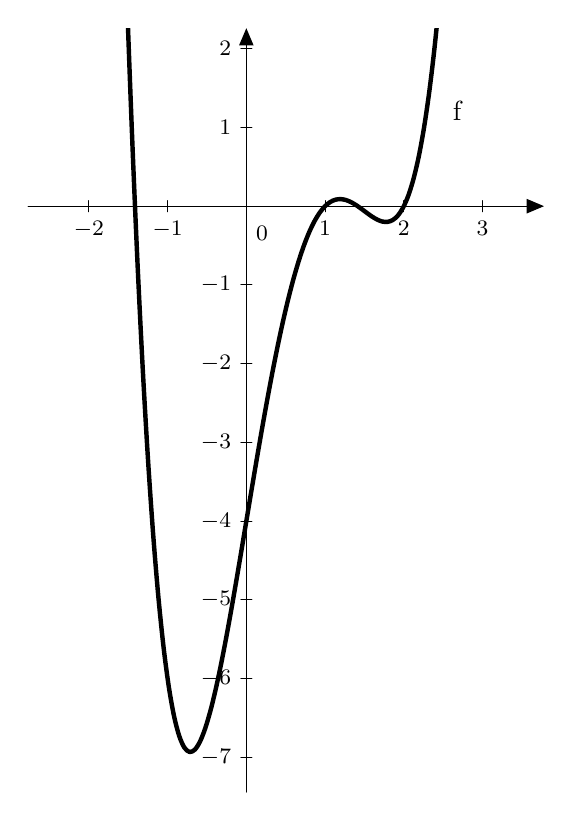
\begin{tikzpicture}[line cap=round,line join=round,>=triangle 45,x=1.0cm,y=1.0cm]
    \draw[->,color=black] (-2.77,0) -- (3.78,0);
    \foreach \x in {-2,-1,1,2,3}
    \draw[shift={(\x,0)},color=black] (0pt,2pt) -- (0pt,-2pt) node[below] {\footnotesize $\x$};
    \draw[->,color=black] (0,-7.44) -- (0,2.26);
    \foreach \y in {-7,-6,-5,-4,-3,-2,-1,1,2}
    \draw[shift={(0,\y)},color=black] (2pt,0pt) -- (-2pt,0pt) node[left] {\footnotesize $\y$};
    \draw[color=black] (0pt,-10pt) node[right] {\footnotesize $0$};
    \clip(-2.77,-7.44) rectangle (3.78,2.26);
    \draw[line width=1.6pt, smooth,samples=100,domain=-2.7709659189295555:3.7776369933097222] plot(\x,{(\x)^4-3*(\x)^3+6*(\x)-4});
    \draw (2.5,1.46) node[anchor=north west] {f};
    \end{tikzpicture}
  \end{center}
  \item $f(x)=x^5-x^4-13x^3+13x^2+36x-36$
  \begin{center}
    \definecolor{cqcqcq}{rgb}{0.75,0.75,0.75}
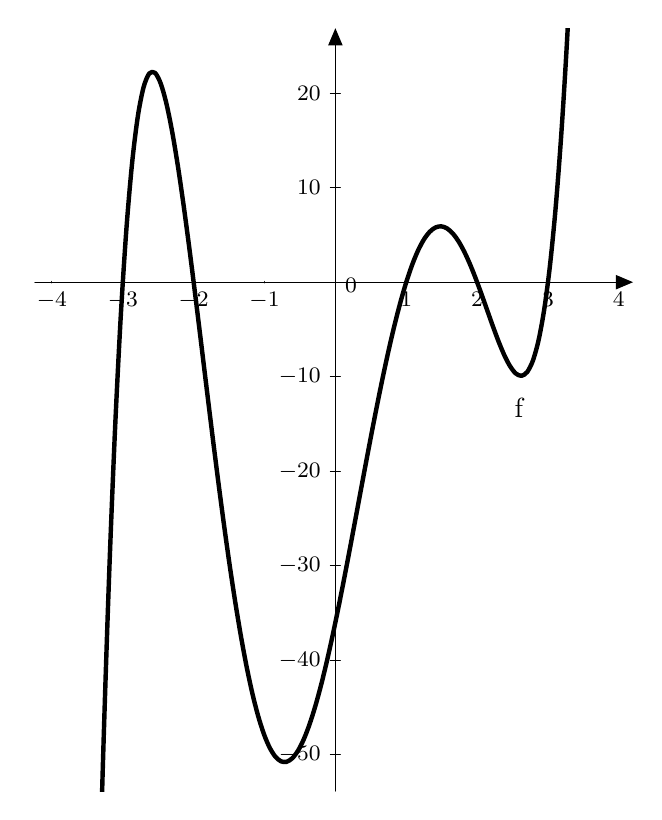
\begin{tikzpicture}[xscale=.9, yscale=.12, line cap=round,line join=round,>=triangle 45,x=1.0cm,y=1.0cm]
\draw[->,color=black] (-4.24,0) -- (4.2,0);
\foreach \x in {-4,-3,-2,-1,1,2,3,4}
\draw[shift={(\x,0)},color=black] (0pt,2pt) -- (0pt,-2pt) node[below] {\footnotesize $\x$};
\draw[->,color=black] (0,-53.86) -- (0,26.88);
\foreach \y in {-50,-40,-30,-20,-10,10,20}
\draw[shift={(0,\y)},color=black] (2pt,0pt) -- (-2pt,0pt) node[left] {\footnotesize $\y$};
\draw[color=black] (0pt,-10pt) node[right] {\footnotesize $0$};
\clip(-4.24,-53.86) rectangle (4.2,26.88);
\draw[line width=1.6pt, smooth,samples=100,domain=-4:4] plot(\x,{(\x)^5-(\x)^4-13*(\x)^3+13*(\x)^2+36*(\x)-36});
\draw (2.39,-11.21) node[anchor=north west] {f};
\end{tikzpicture}
  \end{center}
  \item $f(x)=x^4-\dfrac{23}{12}x^3+\dfrac{29}{24}x^2-\dfrac{1}{4}x$
  \begin{center}
    \definecolor{cqcqcq}{rgb}{0.75,0.75,0.75}
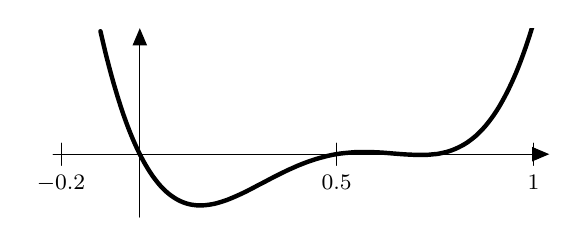
\begin{tikzpicture}[xscale=5, yscale=40,line cap=round,line join=round,>=triangle 45,x=1.0cm,y=1.0cm]
\draw[->,color=black] (-0.22,0) -- (1.04,0);
\foreach \x in {-0.2,0.5,1}
\draw[shift={(\x,0)},color=black] (0pt,.1pt) -- (0pt,-.1pt) node[below] {\footnotesize $\x$};
\draw[->,color=black] (0,-0.02) -- (0,0.04);
\foreach \y in {}
\draw[shift={(0,\y)},color=black] (2pt,0pt) -- (-2pt,0pt) node[left] {\footnotesize $\y$};
\clip(-0.22,-0.02) rectangle (1.04,0.04);
\draw[line width=1.6pt, smooth,samples=100,domain=-0.1:1] plot(\x,{(\x)^4-23/12*(\x)^3+29/24*(\x)^2-1/4*(\x)});
\draw (2.39,-12.67) node[anchor=north west] {f};
\end{tikzpicture}
  \end{center}
  \item $f(x)=x^5-15x^3+10x^2+60x-72$
  \begin{center}
    \definecolor{cqcqcq}{rgb}{0.75,0.75,0.75}
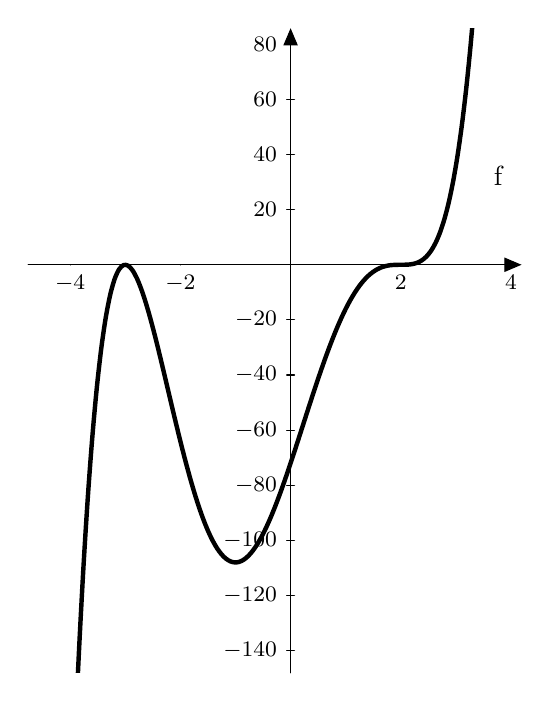
\begin{tikzpicture}[xscale=.7, yscale=.035,line cap=round,line join=round,>=triangle 45,x=1.0cm,y=1.0cm]
\draw[->,color=black] (-4.76,0) -- (4.19,0);
\foreach \x in {-4,-2,2,4}
\draw[shift={(\x,0)},color=black] (0pt,2pt) -- (0pt,-2pt) node[below] {\footnotesize $\x$};
\draw[->,color=black] (0,-148.05) -- (0,85.82);
\foreach \y in {-140,-120,-100,-80,-60,-40,-20,20,40,60,80}
\draw[shift={(0,\y)},color=black] (2pt,0pt) -- (-2pt,0pt) node[left] {\footnotesize $\y$};
\clip(-4.76,-148.05) rectangle (4.19,85.82);
\draw[line width=1.6pt, smooth,samples=100,domain=-4:4] plot(\x,{(\x)^5-15*(\x)^3+10*(\x)^2+60*(\x)-72});
\draw (3.51,39.24) node[anchor=north west] {f};
\end{tikzpicture}
  \end{center}
  \item $f(x)=x^6+2x^5-11x^4-12x^3+36x^2$
  \begin{center}
    \definecolor{cqcqcq}{rgb}{0.75,0.75,0.75}
    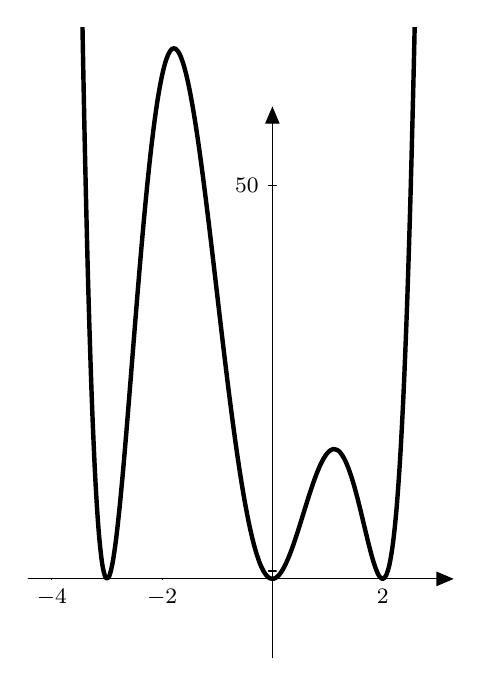
\begin{tikzpicture}[xscale=.7, yscale=.1, line cap=round,line join=round,>=triangle 45,x=1.0cm,y=1.0cm]
    \draw[->,color=black] (-4.43,0) -- (3.29,0);
    \foreach \x in {-4,-2,2}
    \draw[shift={(\x,0)},color=black] (0pt,2pt) -- (0pt,-2pt) node[below] {\footnotesize $\x$};
    \draw[->,color=black] (0,-10) -- (0,60);
    \foreach \y in {,50}
    \draw[shift={(0,\y)},color=black] (2pt,0pt) -- (-2pt,0pt) node[left] {\footnotesize $\y$};
    \clip(-4.43,-10) rectangle (3.29,70);
    \draw[line width=1.6pt, smooth,samples=100,domain=-3.6:2.7] plot(\x,{(\x)^6+2*(\x)^5-11*(\x)^4-12*(\x)^3+36*(\x)^2});
    \draw (-1.44,82.3) node[anchor=north west] {f};
    \end{tikzpicture}
  \end{center}
\end{enumerate}
\end{multicols}
\end{oefening}

\begin{oefening}
Bespreek door gebruik te maken van ICT (domein, bereik, nulwaarden, tekenverloop, stijgen\&dalen):
\begin{enumerate}[(a)]
  \itemsep0.5em
  \item $f(x)=(x-2)^2(x+4)^2$
  \item $f(x)=(x-16)^2-x^2-8x^4-64$
  \item $f(x)=x(x-1)(x-2)(x-3)(x-4)$
  \item $f(x)=-\dfrac{1}{8}(x^4+x^3-14x^2-8x+48)$
\end{enumerate}
\end{oefening}

\begin{oefening}
Beschouw de functie $f(x)=-\dfrac{1}{4}(x^4+3x^3-3x^2-9x)$, met als grafiek:
\begin{center}
\definecolor{cqcqcq}{rgb}{0.75,0.75,0.75}
\begin{tikzpicture}[line cap=round,line join=round,>=triangle 45,x=1.0cm,y=1.0cm]
\draw [color=cqcqcq,dash pattern=on 1pt off 1pt, xstep=1.0cm,ystep=1.0cm] (-4.31,-1.55) grid (3.31,2.64);
\draw[->,color=black] (-4.31,0) -- (3.31,0);
\foreach \x in {-4,-3,-2,-1,1,2,3}
\draw[shift={(\x,0)},color=black] (0pt,2pt) -- (0pt,-2pt) node[below] {\footnotesize $\x$};
\draw[->,color=black] (0,-1.55) -- (0,2.64);
\foreach \y in {-1,1,2}
\draw[shift={(0,\y)},color=black] (2pt,0pt) -- (-2pt,0pt) node[left] {\footnotesize $\y$};
\draw[color=black] (0pt,-10pt) node[right] {\footnotesize $0$};
\clip(-4.31,-1.55) rectangle (3.31,2.64);
\draw[line width=1.6pt, smooth,samples=100,domain=-4.306720586404644:3.3067938031642226] plot(\x,{(-1)/4*((\x)^4+3*(\x)^3-3*(\x)^2-9*(\x))});
\draw (1.54,2.02) node[anchor=north west] {f};
\end{tikzpicture}
\end{center}
Bespreek (domein, bereik, nulwaarden, tekenverloop, stijgen\&dalen).
\end{oefening}

\begin{oefening}
Construeer een veeltermfunctie van de vierde graad met nulwaarden $x_0=-4$, $x_1=2$ en $x_2=3$. De nulwaarde $x_1$ komt tweemaal voor (we zeggen dat deze multipliciteit 2 heeft). De functie moet negatief zijn voor $x\in]-\infty,-4[$.
\end{oefening}


\pagebreak
\section{Veeltermongelijkheden}

\begin{oefening}
Los op in $\mathbb{R}$:
\begin{multicols}{2}
\begin{enumerate}[(a)]
  \itemsep0.6em
  \item $x-5<0$
  \item $2x+3\geq 2$
  \item $8x-3<0$
  \item $7\leq 7-49x$
\end{enumerate}
\end{multicols}
\end{oefening}

\begin{oefening}
Los op in $\mathbb{R}$:
\begin{multicols}{2}
\begin{enumerate}[(a)]
  \itemsep0.6em
  \item $-6x^2+13x-6\leq 0$
  \item $80x^2-20x-10\geq 0$
  \item $-15x^2+30x+45\geq 45$
  \item $x^2+4x+4 < 0$
  \item $(x+2)^2 > 4x$
  \item $-x^2 > -4x$
\end{enumerate}
\end{multicols}
\end{oefening}



\begin{oefening}
Los op in $\mathbb{R}$:
\begin{multicols}{2}
\begin{enumerate}[(a)]
  \itemsep0.6em
  \item $x^2(2-x)\leq6-5x$
  \item $2x^3-x^2-13x<6$
  \item $x(x+2)^2\leq9+x-x^2$
  \item $x(x^2+12)>2(3x^2+4)$
  \item $x(x^2-3)<2$
  \item $x^4+27x^2+4x<36+12x^3$
  \item $12+x^3\geq13x$
  \item $x^4-71x^2-66x-4x^3>0$
  \item $2x(x+1)-\frac{1}{2}x<2(x+1)^2$
  \item $(1+2x)^2\leq(x-2)(x+2)$
  \item $x(x+1)-\frac{x+3}{10}$
  \item $-x^3+2x^2\leq6-5x$
  \item $\frac{x(x^2-3)}{2}<1$
  \item $x^3\geq8$
\end{enumerate}
\end{multicols}
\end{oefening}

\begin{oefening}
Welke reële getallen zijn groter dan hun derdemacht?
\end{oefening}

\begin{oefening}
Voor welke reële getallen is het kwadraat groter dan de derdemacht
\end{oefening}

\begin{oefening}
Heeft elke veeltermongelijkheid oplossingen? Indien je nee antwoord, geef een voorbeeld van een veeltermongelijkheid die geen oplossingen heeft.
\end{oefening}


\pagebreak
\section{Toepassingen}

\begin{oefening}
Kasper heeft na zijn verjaardagsfeest nog een vuurpijl over. Hij vuurt die af vanuit zijn slaapkamer. De pijl vliegt eerst lichtjes naar beneden, maar gaat uiteindelijk toch de lucht in om na 5 seconden te ontploffen. De hoogte $h$ (in meters) in functie van de tijd $x$ (in seconden) wordt beschreven door de formule:
$$h=x^3-4x^2+2x+8$$
\begin{enumerate}[(a)]
  \item Hoe hoog is de slaapkamer van Kasper?
  \item Hoe hoog is de vuurpijl na 5 seconden?
  \item Wanneer vliegt de vuurpijl op een hoogte van 5 meter?
\end{enumerate}
\end{oefening}

\begin{oefening}
De hoogte $h$ (in meters) van een luchtballon $t$ uren na het opstijgen wordt gegeven door de functie:
$$h(t)=-t^4+9t^3-120t^2+500t$$.
\begin{enumerate}[(a)]
  \item Bereken na hoeveel tijd de ballon weer op de grond komt.
  \item Na hoeveel uren vliegt de ballon op een hoogte van 400m?
\end{enumerate}
\end{oefening}

\begin{oefening}
Een bedrijf produceert fietscomputertjes. De bedrijfsleiding wil weten hoeveel computertjes per uur moeten geproduceerd worden om winst te maken in de huidige situatie. Het verband tussen de winst $W$ (in euro) en de productie $x$ (aantal geproduceerde computertjes) per uur is:
$$W(x)=-\dfrac{1}{2}x^3+8x^2-\dfrac{55}{2}x$$
\begin{enumerate}[(a)]
  \item Bij welke productie zal de winst 0 euro bedragen?
  \item Bij welke productie wordt er winst gemaakt?
  \item Bij welke productie wordt er verlies gemaakt?
  \item Bij welke productie is de winst gelijk aan 36 euro?
\end{enumerate}
\end{oefening}

\begin{oefening}
Een game studio modelleert de winst op zijn laatste computer spelletje met behulp van
$$W(n)=-2n^2+28n-90$$ waarbij $n$ het aantal per honderdduizend verkochte spelletjes is en waarbij $W$ de winst is in miljoenen euro.
\begin{enumerate}[(a)]
  \item Hoeveel spelletjes moet het bedrijf op zijn minst verkopen om uit de kosten te geraken?
  \item Wanneer maakt het bedrijf winst/verlies?
\end{enumerate}
\end{oefening}

\begin{oefening}
De bevolking van een Limburgse gemeente is sinds 1980 geëvolueert volgens de functie $$f(x)=5x^3-85x^2+80x+4000$$ waarbij $x=0$ overeenkomt met het jaar 1980.
\begin{enumerate}[(a)]
  \item Hoeveel inwonders waren er in 1980?
  \item In welk jaar zullen er 31000 inwoners zijn? (één tijdstip volstaat)
\end{enumerate}
\end{oefening}

\begin{oefening}
Een groep bergbeklimmers vertrekt op tocht.  De route die zij volgen wordt beschreven	door de volgende veeltermfunctie $$h(x)=90x^2-10x^3$$ met
\begin{itemize}
  \item h = hoogte in meter
  \item x = tijd in uren ( x = 0 is het tijdstip waarop de groep begint met de beklimming)
\end{itemize}
\begin{enumerate}[(a)]
  \item Hoelang duurt de tocht?
  \item Na hoeveel uur bereikt de groep een hoogte van 800 meter? (één tijdstip volstaat)
\end{enumerate}
\end{oefening}

\begin{oefening}
Een bedrijf produceert gps-toestellen voor auto’s.  De bedrijfsleiding wil weten hoeveel toestellen er per uur geproduceerd moeten worden om winst te maken in de huidige situatie.  Het verband tussen de winst $W$ (in euro) en de productie $x$ (aantal geproduceerde toestellen) per uur is
$$W=-\dfrac{3}{2}x^3+24x^2-72x\;.$$
\begin{enumerate}[(a)]
  \item Bij welke productie is de winst gelijk aan 0 euro ($W = 0$)?
  \item Bij welke productie wordt er winst ($W > 0$) en bij welke productie wordt er verlies ($W < 0$) gemaakt?
  \item Bij welke productie is de winst gelijk aan 108 euro?  (één oplossing volstaat)
\end{enumerate}
\end{oefening}

\begin{oefening}
Ibuprofen is een pijnstillend middel.  Om het aantal mg $m$ van het middel in de bloedsomloop te schatten, $t$ uren nadat 100 mg van dit middel werd ingenomen, gebruiken we het verband
$$m(t)=-t^4+4t^3-9t^2+36t$$
met $m =$ aantal $\mg$ van het middel Ibuprofen in het bloed $t = $ aantal uren nadat je $100 \mg$ Ibuprofen hebt ingenomen.
\begin{enumerate}[(a)]
  \item Wanneer is het pijnstillend middel uitgewerkt?
  \item Op welk tijdstip is het opgenomen gehalte in het bloed gelijk aan $30 \mg$? (één tijdstip volstaat)
\end{enumerate}
\end{oefening}

\begin{oefening}
Het aantal bezoekers dat zich op een zonnige dag in de maand juli in een dierenpark bevindt, zou je kunnen benaderen door het functievoorschrift
$$n(t)=100t+140t^2-15t^3$$
met $n(t)$ het aantal bezoekers op tijdstip $t$ in uren, waarbij $t=0$ overeenkomt met 9u 's morgens (het openingsuur van het dierenpark).
\begin{enumerate}[(a)]
  \item Bepaal het sluitingsuur van het dierenpark.
  \item Hoeveel bezoekers waren er om 12 uur 's middags?
\end{enumerate}
\end{oefening}

\begin{oefening}
Stef woont in een appartement en laat van in zijn venster een opgeblazen ballon vliegen.  Deze gaat eerst naar beneden om dan snel de hoogte in te gaan.  De baan kan beschreven worden door de volgende veeltermfunctie
$$h(x)=-4x^3+16x^2-6x+12\;.$$
Hierbij is
\begin{itemize}
  \item $h$ de hoogte in meter,
  \item $x$ de afstand in meter.
\end{itemize}
Hoe hoog is de vensterbank van het raam waaruit Stef de ballon laat vliegen? Duid het juiste antwoord aan en leg uit waarom je die oplossing hebt gekozen.\\
\begin{center}
  \begin{tabular}{|ccccc|}
  \hline
  4 meter & 6 meter & 8 meter & 12 meter & 18 meter\\[0.2cm]
  \hline    
  \end{tabular}
\end{center}
\end{oefening}

\begin{oefening}{\scriptsize\em Opmerking: Deze oefening kon je vorig jaar ook al oplossen want het betreft een tweedegraadsveeltermfunctie}\\
Een ecologische verbindingsbrug moet worden ontworpen over een belangrijke snelweg. De brug over de snelweg wordt gebouwd in de vorm van een parabool. De snelweg is 8 meter breed en wordt gecentreerd onder de parabolische boog. De brug moet in het totaal een breedte van $16 \m$ overspannen. De brug moet een minimale hoogte van 4 m over de snelweg te bieden.
\begin{enumerate}[(a)]
  \item Teken de parabool en de snelweg, label alle relevante afmetingen.
  \item Plaats een coördinatenstelsel op de tekening zodat de $y$-as de snelweg in het midden doorsnijdt en de $x$-as gelegen is aan de voet van de brug.
  \item Vind de kwadratische functie in standaardvorm die de hoogte van de brug $y$ geeft als functie van de horizontale afstand van het centrum $x$.
  \item Bepaal de maximale hoogte van de boog over de snelweg.
\end{enumerate}
\end{oefening}




\end{document}




\begin{minipage}[c]{0.4\textwidth}
\end{minipage}
\begin{minipage}[c]{0.6\textwidth}
\dotlines{10}
\end{minipage}











